\chapter{Diagramma dei casi d'uso}

\section{Registrazione}
\begin{figure}[h!]
\centering
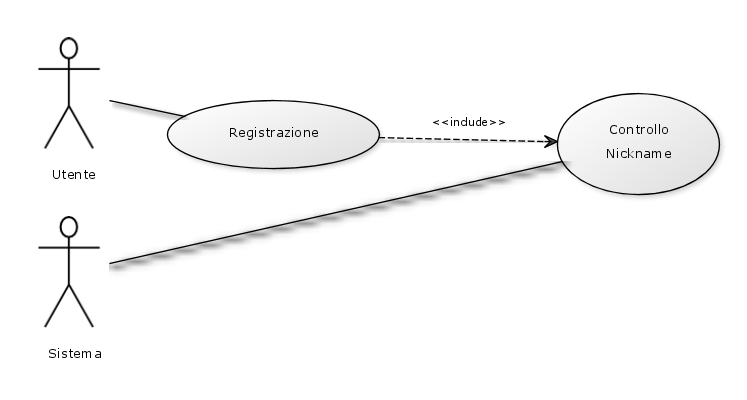
\includegraphics[scale=0.55]{img/registrazione.png}
\caption{Registrazione}
\label{fig:registrazione}
\end{figure}
\begin{table}[H]
\begin{tabular}{p{0.35\textwidth}|p{0.65\textwidth}}
\toprule
%\textbf{Nome} & \textbf{Descrizione} \\
%\midrule
NOME & Registrazione;\\
\hline
OBBIETTIVO: & Registrare l utente nella applicazione;\\
\hline
PRE-CONDIZIONE & L'utente non deve essere registrato nel sistema;\\
\hline
SUCCESSO: & La registrazione avviene con successo;\\
\hline
FALLIMENTO: & Non è possibile effettuare la registrazione; \\
\hline
ATTORE PRIMARIO: & Utente;\\
\hline
ATTORI SECONDARI: & Sistema;\\
\bottomrule
\end{tabular}
\caption{Registrazione}
\label{table:reg}
\end{table}
FLUSSO PRINCIPALE:
\begin{enumerate}
\item L'utente compila e inoltra il modulo d'iscrizione;
\begin{enumerate}
\item Controllo dei campi non opzionali e necessari alla registrazione;
\item Doppio inserimento password;
\end{enumerate}
\item Controllo del nickname;
\item Ricerca del nickname;
\begin{enumerate}
\item Il sistema verifica che l'utente (nickname univoco) non sia già registrato;
\end{enumerate}
\item Avviene la registrazione del utente;
\item La registrazione è avvenuta con successo;
\end{enumerate}
\section{Login}
\begin{figure}[h!]
\centering
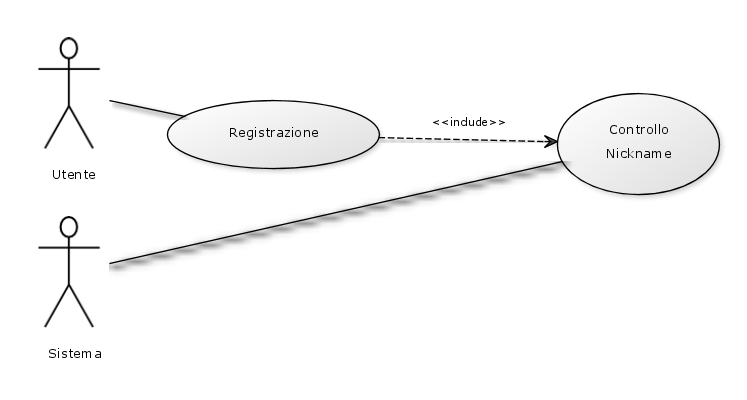
\includegraphics[scale=0.55]{img/registrazione.png}
\caption{Registrazione}
\label{fig:registrazione}
\end{figure}
\begin{table}[H]
\begin{tabular}{p{0.35\textwidth}|p{0.65\textwidth}}
\toprule
%\textbf{Nome} & \textbf{Descrizione} \\
%\midrule
NOME & Login;\\
\hline
OBBIETTIVO: & Ottenere accesso all'applicazione;\\
\hline
PRE-CONDIZIONE & L'Utente deve essere registrato all'applicazione;\\
\hline
SUCCESSO: & L'Utente ottiene accesso all'applicazione;\\
\hline
FALLIMENTO: & La procedura non va a buon fine;\\
\hline
ATTORE PRIMARIO: & Utente;\\
\hline
ATTORI SECONDARI: & Sistema;\\
\bottomrule
\end{tabular}
\caption{Login}
\label{table:log}
\end{table}
FLUSSO PRINCIPALE:
\begin{enumerate}
\item L'Utente immette le proprie credenziali;
\item L'Utente inoltra la richiesta di accesso;
\begin{enumerate}
\item Il sistema verifica la corrispondenza delle credenziali;
\end{enumerate}
\item L'Utente ottiene accesso al' applicazione;
\end{enumerate}

\section{Partecipazione ad evento – Utente senza accesso }
\begin{figure}[h!]
\centering
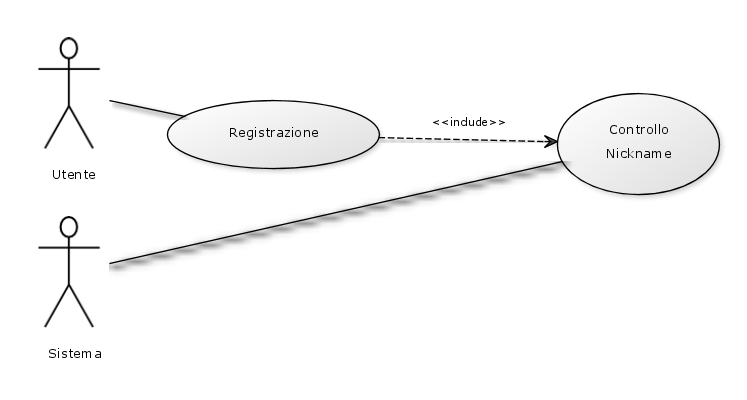
\includegraphics[scale=0.55]{img/registrazione.png}
\caption{Registrazione}
\label{fig:registrazione}
\end{figure}
\begin{table}[H]
\begin{tabular}{p{0.35\textwidth}|p{0.65\textwidth}}
\toprule
%\textbf{Nome} & \textbf{Descrizione} \\
%\midrule
NOME & Partecipazione ad evento senza accesso;\\
\hline
OBBIETTIVO: & L'utente rende la propria disponibilità per un evento senza essere registrato all'applicazione;\\
\hline
PRE-CONDIZIONE & Nessuna;\\
\hline
SUCCESSO: & L utente si rende disponibile per tale evento;\\
\hline
FALLIMENTO: & La procedura non va a buon fine;\\
\hline
ATTORE PRIMARIO: & Utente;\\
\hline
ATTORI SECONDARI: & Sistema;\\
\bottomrule
\end{tabular}
\caption{Partecipazione ad evento senza accesso}
\label{table:par1}
\end{table}
FLUSSO PRINCIPALE:
\begin{enumerate}
\item L'utente seleziona l'evento desiderato e visualizza tutte le informazioni riguardanti l'evento;
\begin{enumerate}
\item L'utente visualizza la lista di tutti gli utenti inscritti all'evento e il nickname dell'utente che l ha creato;
\item L'utente visualizza la lista di tutti i commenti per l evento selezionato;
\end{enumerate}
\item L'Utente inserisce il proprio nome nel apposito spazio;
\begin{enumerate}
\item Il sistema verifica che l'utente ha inserito correttamente il suo nome;
\end{enumerate}
\item L'Utente inoltra la richiesta d inscrizione;
\item L'Utente si rende disponibile per tale evento;
\end{enumerate}

\section{Partecipazione ad evento – Utente con accesso }

\begin{figure}[H]
\centering
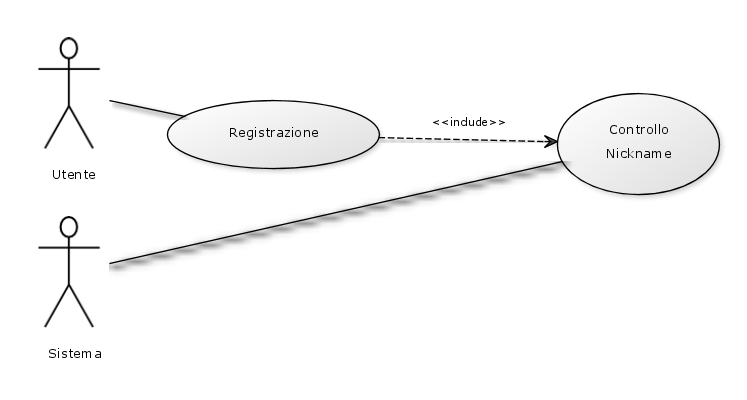
\includegraphics[scale=0.55]{img/registrazione.png}
\caption{Registrazione}
\label{fig:registrazione}
\end{figure}
\begin{table}[H]
\begin{tabular}{p{0.35\textwidth}|p{0.65\textwidth}}
\toprule
%\textbf{Nome} & \textbf{Descrizione} \\
%\midrule
NOME & Partecipazione ad evento con accesso;\\
\hline
OBBIETTIVO: & L'utente rende la propria disponibilità per un evento dopo aver eseguito l'accesso all'applicazione;\\
\hline
PRE-CONDIZIONE & L' Utente deve essere registrato all'applicazione;\\
\hline
SUCCESSO: & L utente si rende disponibile per tale evento;\\
\hline
FALLIMENTO: & La procedura non va a buon fine;\\
\hline
ATTORE PRIMARIO: & Utente;\\
\hline
ATTORI SECONDARI: & Sistema;\\
\bottomrule
\end{tabular}
\caption{Partecipazione ad evento con accesso}
\label{table:par2}
\end{table}

FLUSSO PRINCIPALE:
\begin{enumerate}
\item L'Utente seleziona l'evento desiderato e visualizza tutte le informazioni riguardanti l'evento;
\begin{enumerate}
\item L'Utente visualizza la lista di tutti gli utenti inscritti all'evento e il nickname dell'utente che l ha creato;
\item L'Utente visualizza la lista di tutti i commenti per l evento selezionato;
\end{enumerate}
\item L'Utente inoltra la richiesta d inscrizione;
\begin{enumerate}
\item Il Sistema recupera il nome del utente che ha eseguito l accesso;
\item Il Sistema recupera il nickname del utente che ha eseguito l accesso;
\end{enumerate}
\item L'Utente si rende disponibile per tale evento;
\begin{enumerate}
\item L'utente può lasciare commenti per l evento selezionato;
\end{enumerate}
\end{enumerate}

\section{Chiusura evento}
\begin{figure}[H]
\centering
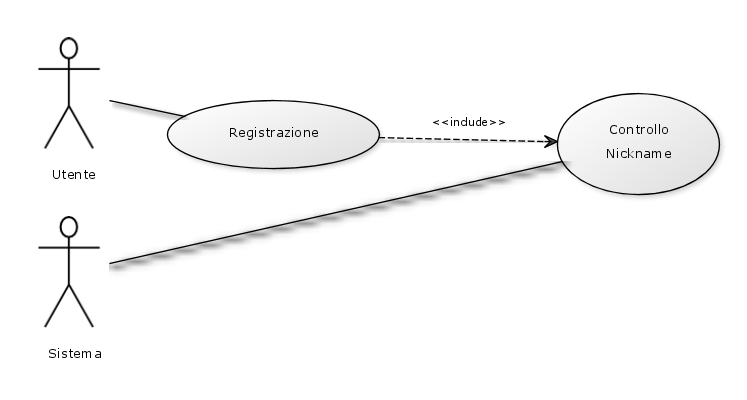
\includegraphics[scale=0.55]{img/registrazione.png}
\caption{Registrazione}
\label{fig:registrazione}
\end{figure}
\begin{table}[H]
\begin{tabular}{p{0.35\textwidth}|p{0.65\textwidth}}
\toprule
%\textbf{Nome} & \textbf{Descrizione} \\
%\midrule
NOME & Chiusura di un evento;\\
\hline
OBBIETTIVO: & L utente chiude un evento;\\
\hline
PRE-CONDIZIONE & L'Utente deve essere registrato all'applicazione;
L'Utente è il creatore dell'evento;\\
\hline
SUCCESSO: & L utente chiude correttamente l evento;\\
\hline
FALLIMENTO: & La procedura non va a buon fine;\\
\hline
ATTORE PRIMARIO: & Utente;\\
\hline
ATTORI SECONDARI: & Sistema;\\
\bottomrule
\end{tabular}
\caption{Chiusura di un evento}
\label{table:chiude}
\end{table}	

FLUSSO PRINCIPALE:
\begin{enumerate}
\item L' utente seleziona l'evento desiderato;
\item L' utente inserisce le eventuali cause che hanno portato alla chiusura dell'evento;
\item L'utente inoltra la richiesta di chiusura dell'evento;
\begin{enumerate}
\item Il Sistema controlla che l'utente che vuole chiudere l evento sia il creatore dello stesso;
\end{enumerate}
\item L utente ha chiuso l'evento;
\end{enumerate}


\section{Eliminazione evento}
\begin{figure}[H]
\centering
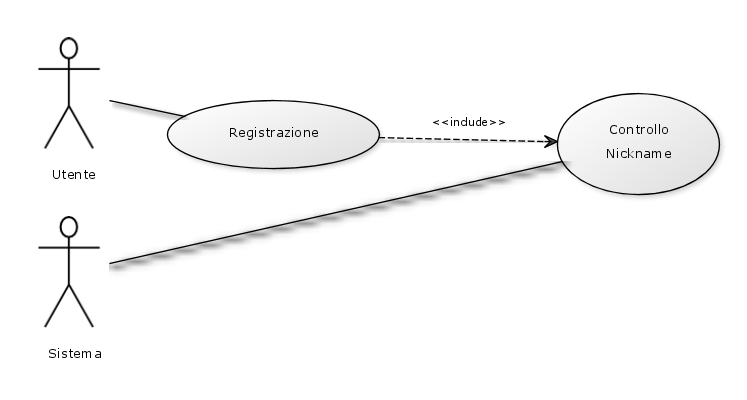
\includegraphics[scale=0.55]{img/registrazione.png}
\caption{Registrazione}
\label{fig:registrazione}
\end{figure}
\begin{table}[H]
\begin{tabular}{p{0.35\textwidth}|p{0.65\textwidth}}
\toprule
%\textbf{Nome} & \textbf{Descrizione} \\
%\midrule
NOME & Eliminazione di un evento;\\
\hline
OBBIETTIVO: & L utente elimina un evento;\\
\hline
PRE-CONDIZIONE & L' Utente deve essere registrato all'applicazione;
L'Utente è il creatore dell'evento;\\
\hline
SUCCESSO: & L utente elimina correttamente l evento;\\
\hline
FALLIMENTO: & La procedura non va a buon fine;\\
\hline
ATTORE PRIMARIO: & Utente;\\
\hline
ATTORI SECONDARI: & Sistema;\\
\bottomrule
\end{tabular}
\caption{Chiusura di un evento}
\label{table:chiude}
\end{table}	

FLUSSO PRINCIPALE:
\begin{enumerate}
\item L'utente seleziona l'evento desiderato;
\item L'utente inoltra la richiesta di eliminazione dell'evento;
\begin{enumerate}
\item Il sistema controlla che l'utente che vuole eliminare l evento sia il creatore dello stesso;
\end{enumerate}
\item L'utente ha eliminato l'evento;
\item L utente ha chiuso l'evento;
\end{enumerate}


\section{Diagramma casi d'uso completo}
\begin{figure}[H]
\centering
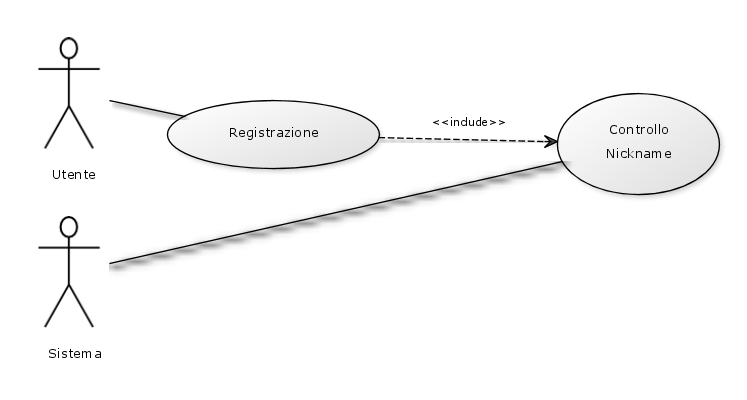
\includegraphics[scale=0.55]{img/registrazione.png}
\caption{Registrazione}
\label{fig:registrazione}
\end{figure}


